\documentclass[11pt]{article}
\usepackage[a4paper,margin=1in]{geometry}
\usepackage[T1]{fontenc}
\usepackage[utf8]{inputenc}
\usepackage{lmodern}
\usepackage{microtype}
\usepackage{amsmath,amssymb,amsthm,mathtools}
\usepackage{bm}
\usepackage{graphicx}
\usepackage{booktabs}
\usepackage{enumitem}
\usepackage{hyperref}
\usepackage[nameinlink,capitalise,noabbrev]{cleveref}
\usepackage{xcolor}
\usepackage{float}

\hypersetup{
  colorlinks=true,
  linkcolor=blue!60!black,
  citecolor=blue!60!black,
  urlcolor=blue!60!black,
  pdftitle={Optimal Geometric Charts for Anchored Divided-Difference Iterations},
  pdfauthor={Ivan Besevic}
}

\newtheorem{theorem}{Theorem}[section]
\newtheorem{proposition}[theorem]{Proposition}
\newtheorem{corollary}[theorem]{Corollary}
\theoremstyle{definition}
\newtheorem{definition}[theorem]{Definition}
\newtheorem{remark}[theorem]{Remark}
\newtheorem{example}[theorem]{Example}

\newcommand{\C}{\mathbb{C}}
\newcommand{\R}{\mathbb{R}}
\newcommand{\dd}{\,\mathrm{d}}
\newcommand{\PF}{P_{F,a}}
\newcommand{\Pphi}{P_{\phi,a}}
\newcommand{\Fphi}{F_{\phi}}
\newcommand{\Oterm}{\mathcal{O}}

\title{Optimal Geometric Charts for Anchored Divided-Difference Iterations\\
\large Local Linearization, Curvature Cancellation, and Jet-Optimal Preconditioning}
\author{Ivan Besevic\\Independent Mathematical Research\\\texttt{github.com/ivan-fr/poussiere\_de\_x}}
\date{May 2026}

\begin{document}
\maketitle

\begin{abstract}
Anchored Pandrosion for a scalar analytic equation $G(z)=0$ can be written, in a chart $\phi$, as the fixed-anchor divided-difference map
\[
P_{\phi,a}(s)=a-\frac{G(\phi(a))}{(G\circ \phi)[a,s]}.
\]
The local behavior of the raw fixed-anchor iteration is therefore determined by the transformed equation $F_{\phi}=G\circ\phi$. This note develops a geometric theory of chart choice. At a simple root $\rho$ with root coordinate $r=\phi^{-1}(\rho)$,
\[
P'_{\phi,a}(r)=1-\frac{F'_{\phi}(r)}{F_{\phi}[a,r]},
\qquad
P'_{\phi,a}(r)=\frac{F''_{\phi}(r)}{2F'_{\phi}(r)}(a-r)+\Oterm((a-r)^2)
\quad (a\to r).
\]
Hence chart optimization is equivalent to flattening $F_{\phi}$ near the root. We prove a first-order optimality criterion: among root-normalized charts, the linear multiplier becomes $\Oterm((a-r)^2)$ if and only if $F''_{\phi}(r)=0$, equivalently
\[
G''(\rho)(\phi'(r))^2+G'(\rho)\phi''(r)=0.
\]
This identifies a curvature-balancing law for the chart. We also show that the local inverse chart of $G$ linearizes the transformed equation exactly and yields one-step convergence, while its quadratic jet gives a canonical practical approximation. Python-generated figures for $G(z)=e^z-2$ illustrate the difference between affine, curvature-balanced, and exact inverse charts. The main message is conceptual: before iterating, choose coordinates in which the transformed equation is as linear as possible.
\end{abstract}

\section{Introduction}
The monomial Pandrosion scheme and its later analytic fixed-anchor formulation show that the essential denominator is a divided difference, not a derivative. In the general scalar analytic setting, one studies
\[
P_{F,a}(s)=a-\frac{F(a)}{F[a,s]},
\qquad
F[a,s]=\frac{F(a)-F(s)}{a-s},
\]
with a fixed anchor $a$ satisfying $F(a)\neq 0$. The local residual factor at a simple root is explicit, and in the analytic continuation paper this residual law was transported through coordinate charts. The natural next question is therefore geometric rather than algorithmic:
\begin{quote}
\emph{Which charts make the anchored divided-difference map as contractive as possible?}
\end{quote}

This question is not cosmetic. In the raw fixed-anchor iteration, the multiplier is linear in the anchor distance. A well-chosen chart can reduce the coefficient of that linear term, or even cancel it. The central idea of the present note is that chart optimization should be read as \emph{local linearization of the transformed equation}. Once the equation is made flat enough in the chosen coordinates, the anchored iteration inherits the improvement automatically.

The paper is local and deliberately modest. It does not claim a global best chart for arbitrary nonlinear equations. Instead, it gives a local geometric criterion, an ideal inverse-chart model, a canonical second-order jet approximation, and a numerical illustration.

\paragraph{Main contributions.}
Let $G$ be analytic near a simple zero $\rho$. The results below establish the following.
\begin{enumerate}[label=(\roman*)]
    \item The charted anchored multiplier depends only on $F_{\phi}=G\circ\phi$.
    \item Among root-normalized charts, first-order optimality is equivalent to $F''_{\phi}(r)=0$.
    \item This is equivalent to a curvature-balancing condition
    \[
    G''(\rho)(\phi'(r))^2+G'(\rho)\phi''(r)=0.
    \]
    \item The local inverse chart of $G$ gives the ideal model $F_{\phi}(s)=s-r$, hence one-step anchored convergence.
    \item The quadratic jet of that inverse is the canonical first nontrivial approximation to the ideal chart.
\end{enumerate}

\section{Anchored divided differences in a chart}
Let $U\subset \C$ be a domain, let $F:U\to\C$ be analytic and nonconstant, and let $a\in U$ satisfy $F(a)\neq 0$.

\begin{definition}[Anchored divided-difference map]
The anchored fixed-point map associated with $(F,a)$ is
\begin{equation}\label{eq:anchored-map}
P_{F,a}(s)=a-\frac{F(a)}{F[a,s]},
\qquad
F[a,s]=\frac{F(a)-F(s)}{a-s},
\end{equation}
where $F[a,a]=F'(a)$ is inserted at the removable point.
\end{definition}

Now let $G$ be analytic on a domain $\Omega\subset\C$, let $\phi:V\to\Omega$ be a local biholomorphic chart, and define
\[
F_{\phi}(s)=G(\phi(s)).
\]
Fix an anchor $a\in V$ such that $G(\phi(a))\neq 0$. The charted anchored map is simply the anchored map for $F_{\phi}$:
\begin{equation}\label{eq:charted-map}
P_{\phi,a}(s)=a-\frac{G(\phi(a))}{F_{\phi}[a,s]}.
\end{equation}
Thus all local questions reduce to the transformed equation $F_{\phi}$.

\begin{proposition}[Exact multiplier and local expansion]\label{prop:exactmultiplier}
Let $F$ be analytic near a simple zero $r$, let $F(a)\neq 0$, and let $a\neq r$. Then $r$ is a fixed point of $P_{F,a}$ and
\begin{equation}\label{eq:multiplier-exact}
P'_{F,a}(r)=1-\frac{F'(r)}{F[a,r]}.
\end{equation}
Moreover, as $a\to r$,
\begin{equation}\label{eq:multiplier-local}
P'_{F,a}(r)=\frac{F''(r)}{2F'(r)}(a-r)+\Oterm((a-r)^2).
\end{equation}
\end{proposition}

\begin{proof}
The fixed-point claim and the exact formula are standard for the fixed-anchor secant map: if $F(r)=0$ then $F[a,r]=F(a)/(a-r)$ and substitution gives $P_{F,a}(r)=r$. Differentiating \eqref{eq:anchored-map} at $r$ yields \eqref{eq:multiplier-exact}. For the local expansion, write
\[
F(a)=F'(r)(a-r)+\frac{F''(r)}{2}(a-r)^2+\Oterm((a-r)^3),
\]
so that
\[
\frac{(a-r)F'(r)}{F(a)}=1-\frac{F''(r)}{2F'(r)}(a-r)+\Oterm((a-r)^2).
\]
Since $P'_{F,a}(r)=1-(a-r)F'(r)/F(a)$, formula \eqref{eq:multiplier-local} follows.
\end{proof}

Applied to $F_{\phi}=G\circ\phi$, this gives
\begin{equation}\label{eq:chart-multiplier}
P'_{\phi,a}(r)=\frac{F''_{\phi}(r)}{2F'_{\phi}(r)}(a-r)+\Oterm((a-r)^2),
\qquad r=\phi^{-1}(\rho),\ \ G(\rho)=0.
\end{equation}
This already identifies the correct optimization target: the chart should make $F''_{\phi}(r)$ small.

\section{Root-normalized charts and first-order optimality}
The right class of coordinates is obtained by normalizing the first jet at the root.

\begin{definition}[Root-normalized chart]
Let $\rho$ be a simple zero of $G$. A local chart $\phi$ is \emph{root-normalized at $\rho$} if there exists a coordinate $r\in V$ such that
\[
\phi(r)=\rho,
\qquad
F'_{\phi}(r)=G'(\rho)\phi'(r)=1.
\]
Equivalently, in the chart coordinate the transformed equation has unit first derivative at the root.
\end{definition}

For a root-normalized chart, Taylor expansion gives
\begin{equation}\label{eq:Fphi-jet}
F_{\phi}(s)=(s-r)+\frac{F''_{\phi}(r)}{2}(s-r)^2+\frac{F'''_{\phi}(r)}{6}(s-r)^3+\Oterm((s-r)^4).
\end{equation}
Hence the coefficient $F''_{\phi}(r)/2$ is the first nonlinear defect of the transformed equation.

\begin{theorem}[First-order optimality criterion]\label{thm:optimality}
Let $G$ be analytic near a simple zero $\rho$, and let $\phi$ be a root-normalized chart with root coordinate $r$. The following are equivalent.
\begin{enumerate}[label=(\alph*)]
    \item $P'_{\phi,a}(r)=\Oterm((a-r)^2)$ as $a\to r$.
    \item $F''_{\phi}(r)=0$.
    \item The chart satisfies the curvature-balancing identity
    \begin{equation}\label{eq:curvature-balance}
    G''(\rho)(\phi'(r))^2+G'(\rho)\phi''(r)=0.
    \end{equation}
\end{enumerate}
In that case the transformed equation is linear up to third order:
\[
F_{\phi}(s)=(s-r)+\Oterm((s-r)^3).
\]
\end{theorem}

\begin{proof}
For a root-normalized chart, \eqref{eq:chart-multiplier} becomes
\[
P'_{\phi,a}(r)=\frac{F''_{\phi}(r)}{2}(a-r)+\Oterm((a-r)^2).
\]
Thus (a) is equivalent to $F''_{\phi}(r)=0$, which proves $(a)\Leftrightarrow (b)$. Next,
\[
F''_{\phi}(r)=G''(\rho)(\phi'(r))^2+G'(\rho)\phi''(r)
\]
by the chain rule. Hence $F''_{\phi}(r)=0$ is exactly \eqref{eq:curvature-balance}, proving $(b)\Leftrightarrow (c)$. The final claim follows from the Taylor expansion \eqref{eq:Fphi-jet}.
\end{proof}

\begin{remark}[Geometric meaning]
The quantity $\phi''/\phi'$ is the logarithmic curvature of the chart. Theorem~\ref{thm:optimality} says that the chart should bend so as to cancel the quadratic curvature of the original equation. Affine scaling can change the size of the multiplier, but a genuinely curved chart is needed to cancel the first nonlinear defect unless $G''(\rho)=0$ already.
\end{remark}

\begin{corollary}[Canonical quadratic jet]\label{cor:quadratic-jet}
Let $G$ be analytic near a simple zero $\rho$, and choose the root coordinate $r=0$. The quadratic jet
\begin{equation}\label{eq:jet-optimal}
\phi_{\mathrm{jet}}(s)=\rho+\frac{s}{G'(\rho)}-\frac{G''(\rho)}{2G'(\rho)^3}s^2+\Oterm(s^3)
\end{equation}
is root-normalized and first-order optimal. It is the unique quadratic jet with these two properties.
\end{corollary}

\begin{proof}
The root-normalization imposes $\phi(0)=\rho$ and $\phi'(0)=1/G'(\rho)$. Theorem~\ref{thm:optimality} then forces
\[
\phi''(0)=-\frac{G''(\rho)}{G'(\rho)^3}.
\]
This uniquely determines the quadratic jet.
\end{proof}

\section{The ideal inverse chart}
The previous section gives a second-order criterion. There is also an ideal local model.

\begin{theorem}[Exact linearization by the local inverse chart]\label{thm:inversechart}
Let $G$ be analytic near a simple zero $\rho$. Then there exists a local inverse $\Psi$ of $G$ near $0$ with $\Psi(0)=\rho$. If one defines, in a root coordinate with $r=0$,
\begin{equation}\label{eq:exact-inverse-chart}
\phi_*(s)=\Psi(s),
\end{equation}
then
\[
F_{\phi_*}(s)=G(\phi_*(s))=s
\]
exactly on a neighborhood of $0$. Consequently, for every anchor $a$ in that neighborhood,
\[
P_{\phi_*,a}(s)=0
\]
for all $s$ where the map is defined. In the ideal inverse chart, anchored iteration converges in one step.
\end{theorem}

\begin{proof}
Since $G'(\rho)\neq 0$, the inverse function theorem gives a local inverse $\Psi$ with $G(\Psi(s))=s$. Hence $F_{\phi_*}(s)=s$. Its divided difference is identically $1$, so
\[
P_{\phi_*,a}(s)=a-\frac{F_{\phi_*}(a)}{F_{\phi_*}[a,s]}=a-a=0.
\]
\end{proof}

\begin{remark}[Interpretation]
The exact inverse chart is not usually available in closed form for a general analytic equation. Nevertheless, it provides the correct conceptual target: the best chart is the one that makes the transformed equation as close as possible to the identity map. Corollary~\ref{cor:quadratic-jet} is precisely the second-order truncation of this ideal model.
\end{remark}

A simple one-parameter family already exhibits the optimization mechanism.

\begin{proposition}[Quadratic family]\label{prop:quadratic-family}
Assume $r=0$ and let
\begin{equation}\label{eq:quadfamily}
\phi_{\eta}(s)=\rho+\frac{s}{G'(\rho)}+\eta s^2.
\end{equation}
Then $\phi_{\eta}$ is root-normalized for every $\eta$, and the first-order multiplier coefficient is
\begin{equation}\label{eq:ceta-general}
P'_{\phi_\eta,a}(0)=c_\eta\, a+\Oterm(a^2),
\qquad
c_\eta=\frac{G''(\rho)}{2G'(\rho)^2}+\eta G'(\rho).
\end{equation}
The unique first-order optimal parameter is
\begin{equation}\label{eq:eta-opt}
\eta_*=-\frac{G''(\rho)}{2G'(\rho)^3}.
\end{equation}
\end{proposition}

\begin{proof}
Since $\phi_\eta(0)=\rho$ and $\phi'_\eta(0)=1/G'(\rho)$, the family is root-normalized. Moreover,
\[
\phi''_\eta(0)=2\eta.
\]
Substituting this into \eqref{eq:curvature-balance} yields
\[
F''_{\phi_\eta}(0)=\frac{G''(\rho)}{G'(\rho)^2}+2\eta G'(\rho),
\]
so the coefficient in \eqref{eq:chart-multiplier} is exactly $c_\eta=F''_{\phi_\eta}(0)/2$. Setting $c_\eta=0$ gives \eqref{eq:eta-opt}.
\end{proof}

\section{Numerical illustration: \texorpdfstring{$G(z)=e^z-2$}{G(z)=exp(z)-2}}
We now illustrate the theory on the simple analytic equation
\[
G(z)=e^z-2,
\qquad
\rho=\log 2.
\]
Since $G'(\rho)=G''(\rho)=2$, the root-normalized affine chart is
\[
\phi_{\mathrm{aff}}(s)=\rho+\frac{s}{2},
\]
and the first-order optimal quadratic jet from \eqref{eq:jet-optimal} is
\[
\phi_{\mathrm{opt}}(s)=\rho+\frac{s}{2}-\frac{s^2}{8}.
\]
The ideal inverse chart is explicit here because the inverse of $e^z-2$ near $0$ is
\[
\phi_*(s)=\log(2+s).
\]
Therefore
\[
F_{\mathrm{aff}}(s)=2e^{s/2}-2=s+\frac{s^2}{4}+\Oterm(s^3),
\]
\[
F_{\mathrm{opt}}(s)=2e^{s/2-s^2/8}-2=s-\frac{s^3}{24}+\Oterm(s^4),
\]
\[
F_*(s)=s.
\]
The affine chart leaves a quadratic defect, the optimal quadratic chart cancels it, and the inverse chart removes it exactly.

\begin{figure}[H]
    \centering
    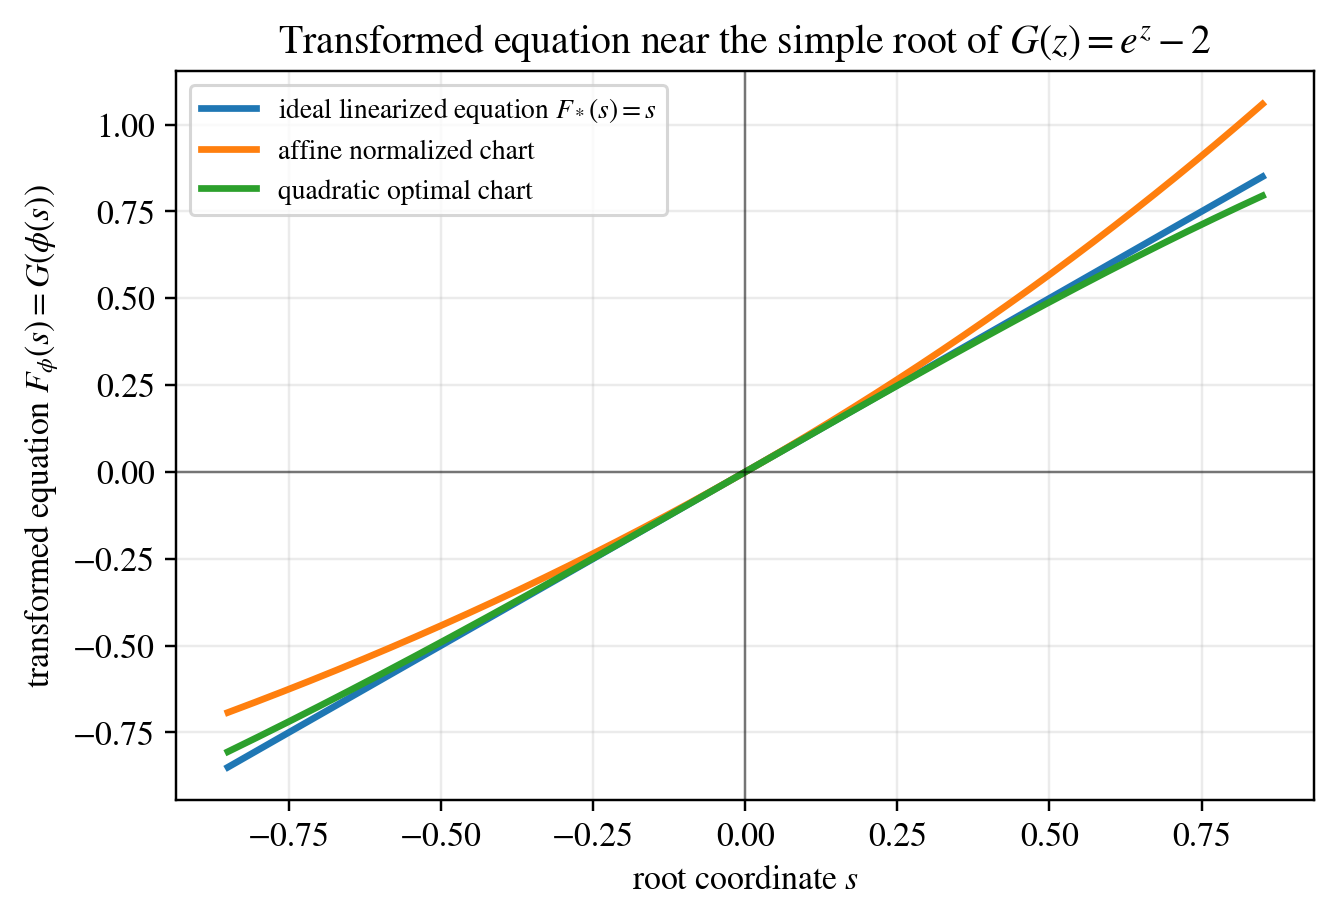
\includegraphics[width=.78\textwidth]{../figures/fig_transformed_equation_profiles.png}
    \caption{Transformed equations for the affine normalized chart, the curvature-balanced quadratic chart, and the ideal linearized model. The optimal chart is visibly flatter at the root.}
    \label{fig:profiles}
\end{figure}

For the quadratic family
\[
\phi_\eta(s)=\rho+\frac{s}{2}+\eta s^2,
\]
\cref{prop:quadratic-family} gives
\[
c_\eta=\frac14+2\eta,
\]
so the optimal parameter is $\eta_*=-1/8$.

\begin{figure}[H]
    \centering
    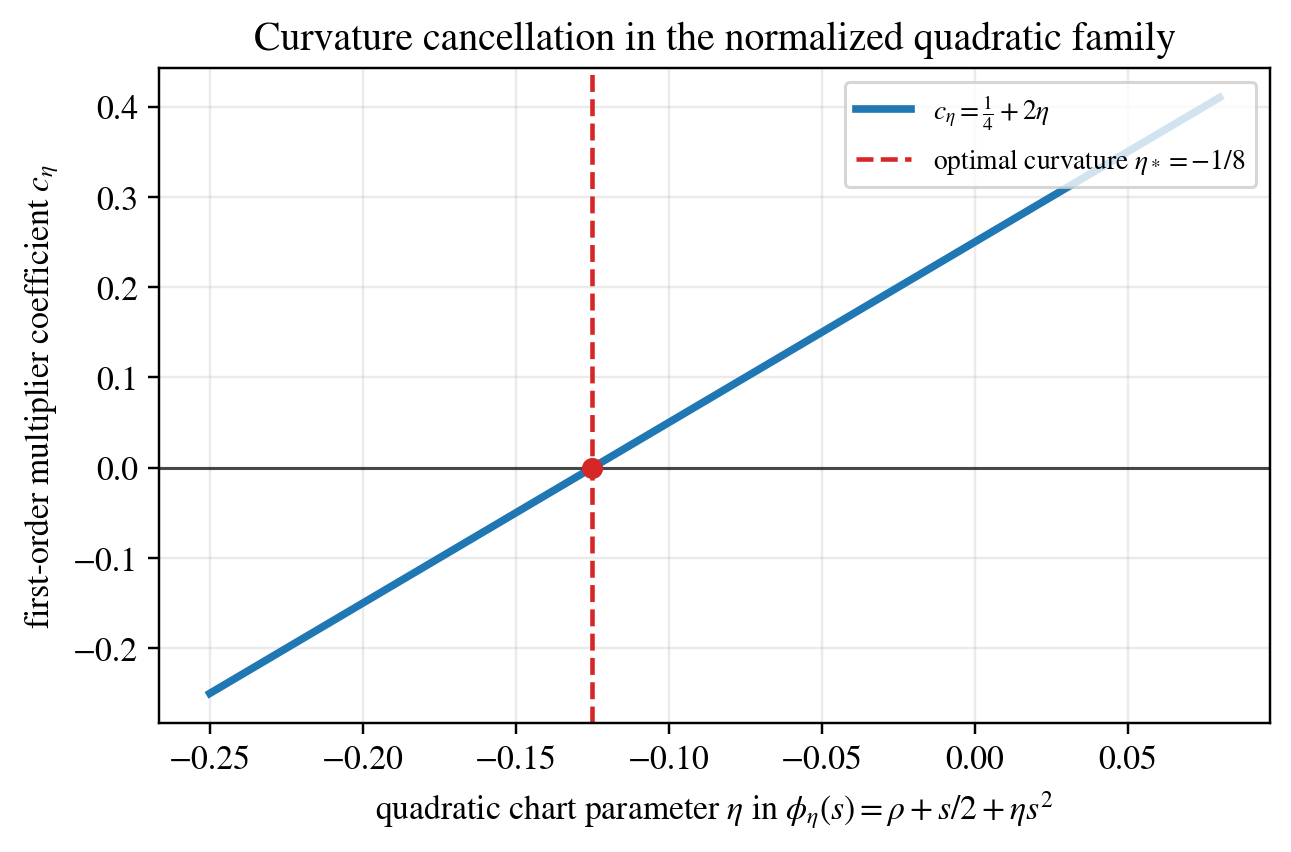
\includegraphics[width=.74\textwidth]{../figures/fig_curvature_balance.png}
    \caption{The first-order multiplier coefficient $c_\eta$ in the quadratic chart family. The zero crossing at $\eta=-1/8$ is the curvature-balancing law.}
    \label{fig:curvature}
\end{figure}

Next, we compare the exact multiplier $\lambda_\phi(h)=P'_{\phi,a}(0)$ with anchor distance $h=|a|$. For the affine chart, $|\lambda_\phi(h)|\asymp h$. For the curvature-balanced chart, $|\lambda_\phi(h)|\asymp h^2$, exactly as predicted by Theorem~\ref{thm:optimality}.

\begin{figure}[H]
    \centering
    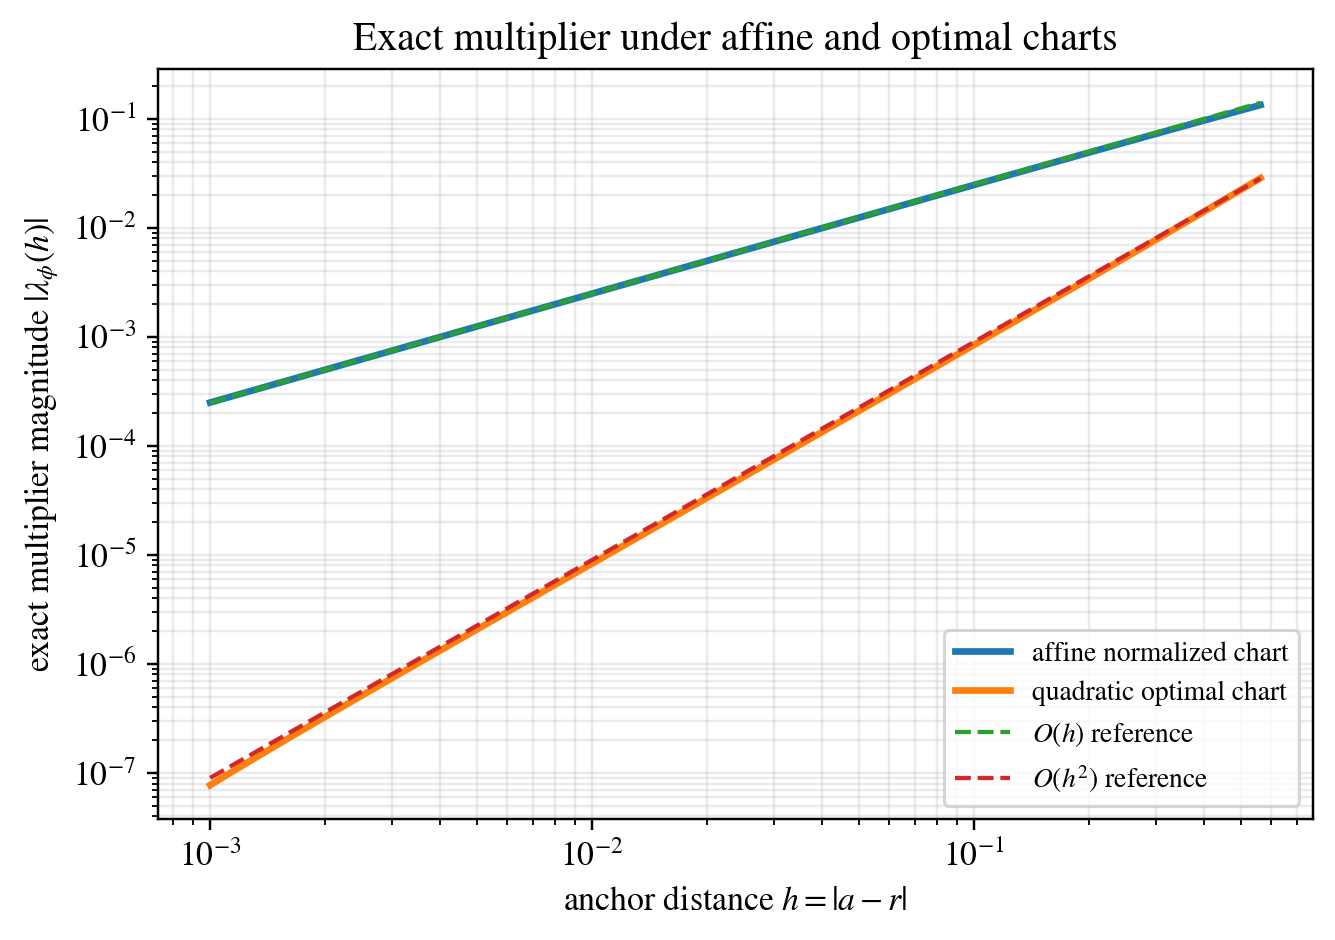
\includegraphics[width=.80\textwidth]{../figures/fig_multiplier_vs_anchor.png}
    \caption{Exact multiplier magnitude versus anchor distance. The affine chart has linear behavior, while the optimal quadratic chart exhibits quadratic decay.}
    \label{fig:multiplier}
\end{figure}

Finally, with anchor $a=0.3$ and start $s_0=0.6$, the fixed-anchor orbits behave as follows.

\begin{table}[H]
    \centering
    \begin{tabular}{lccc}
    \toprule
    chart & $|\lambda_\phi(0.3)|$ & iterations to $|s_n|\le 10^{-12}$ & comment \\
    \midrule
    affine normalized & $7.3126\times 10^{-2}$ & 11 & linear regime \\
    optimal quadratic & $7.8149\times 10^{-3}$ & 6 & improved by curvature cancellation \\
    exact inverse & $0$ & 1 & ideal one-step model \\
    \bottomrule
    \end{tabular}
    \caption{Fixed-anchor comparison for $G(z)=e^z-2$, anchor $a=0.3$, and start $s_0=0.6$.}
    \label{tab:counts}
\end{table}

\begin{figure}[H]
    \centering
    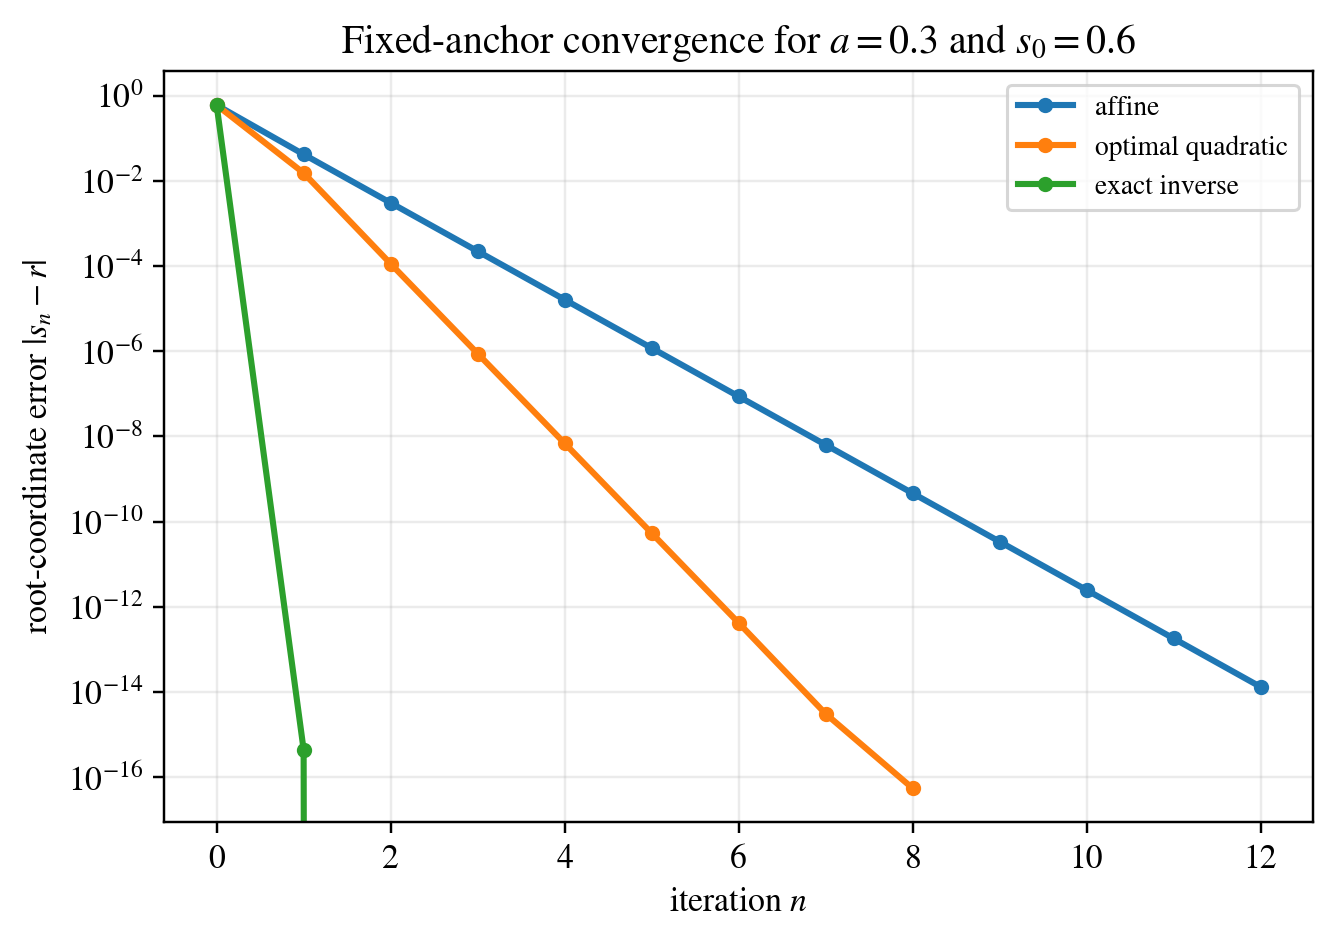
\includegraphics[width=.80\textwidth]{../figures/fig_error_histories.png}
    \caption{Root-coordinate errors for the same test problem. The curvature-balanced chart shortens the linear regime substantially, while the exact inverse chart collapses the problem in one step.}
    \label{fig:errors}
\end{figure}

The point of these figures is not raw speed in the Newton-versus-Pandrosion sense. The point is that the chart alone changes the local geometry of the transformed equation, and the anchored iteration simply reflects that geometric change.

\section{Discussion and outlook}
The local inverse chart shows what ``optimal'' means in principle: the transformed equation should be as close as possible to the identity. The first-order optimality criterion then supplies the practical surrogate: cancel the quadratic defect of the transformed equation. This produces a clear geometric hierarchy.
\begin{enumerate}[label=(\arabic*)]
    \item \textbf{Affine scaling} changes the size of the multiplier coefficient.
    \item \textbf{Curved chart optimization} can cancel the first nonlinear defect entirely.
    \item \textbf{Exact inverse charts} give perfect local linearization when available.
\end{enumerate}

This suggests several continuations.
\begin{itemize}
    \item \textbf{Adaptive chart selection.} Instead of fixing one chart, one could update a local jet approximation of the inverse along the orbit.
    \item \textbf{Anchor--chart co-optimization.} The multiplier depends on both the anchor and the transformed equation. A natural next step is to optimize them jointly.
    \item \textbf{Several variables.} In higher dimension, the same viewpoint would replace scalar curvature cancellation by cancellation of the quadratic tensor in a root-normalized coordinate system.
\end{itemize}

The present note is therefore best read as a geometric preconditioning principle for anchored divided-difference iterations: before iterating, choose coordinates that flatten the transformed equation.

\section*{Acknowledgments}
The figures in this manuscript were generated in Python with Matplotlib and incorporated into the final manuscript via \LaTeX. The present note is intended as a continuation of the monomial and general anchored Pandrosion manuscripts.

\begin{thebibliography}{10}

\bibitem{BesevicMonomial}
I.~Besevic,
\newblock \emph{A Monomial Pandrosion Scheme: Contraction, Chart Scaling, and Steffensen Acceleration for $z^p=x$},
\newblock Independent Mathematical Research, manuscript, May 2026.

\bibitem{BesevicAnchored}
I.~Besevic,
\newblock \emph{Anchored Pandrosion for General Analytic Equations: Divided-Difference Fixed Points, Chart Selection, and Steffensen Acceleration},
\newblock Independent Mathematical Research, manuscript, May 2026.

\bibitem{Aitken}
A.~C. Aitken,
\newblock On Bernoulli's numerical solution of algebraic equations,
\newblock \emph{Proc. Roy. Soc. Edinburgh} \textbf{46} (1926), 289--305.

\bibitem{Steffensen}
J.~F. Steffensen,
\newblock Remarks on iteration,
\newblock \emph{Skandinavisk Aktuarietidskrift} \textbf{16} (1933), 64--72.

\bibitem{Traub}
J.~F. Traub,
\newblock \emph{Iterative Methods for the Solution of Equations},
\newblock Prentice--Hall, 1964.

\bibitem{Householder}
A.~S. Householder,
\newblock \emph{The Numerical Treatment of a Single Nonlinear Equation},
\newblock McGraw--Hill, 1970.

\bibitem{OrtegaRheinboldt}
J.~M. Ortega and W.~C. Rheinboldt,
\newblock \emph{Iterative Solution of Nonlinear Equations in Several Variables},
\newblock Academic Press, 1970.

\bibitem{Ostrowski}
A.~M. Ostrowski,
\newblock \emph{Solution of Equations and Systems of Equations},
\newblock 2nd ed., Academic Press, 1966.

\end{thebibliography}

\end{document}
